\documentclass[11pt,a4paper]{article}

\usepackage[T1]{fontenc}
\usepackage{lmodern}
\usepackage[margin=2.45cm,headheight=15pt]{geometry}
\usepackage[spanish,es-nodecimaldot]{babel}
\usepackage{amsmath,amssymb}
\usepackage{graphicx}
\usepackage{booktabs}
\usepackage{tabularx}
\usepackage{array}
\usepackage{caption}
\usepackage{float}
\usepackage{microtype}
\usepackage{setspace}
\usepackage{enumitem}
\usepackage{natbib}
\usepackage{xcolor}
\usepackage{fancyhdr}
\usepackage{hyperref}
\usepackage{url}

\definecolor{azulUCU}{HTML}{123D72}
\hypersetup{
  colorlinks=true,
  linkcolor=azulUCU,
  citecolor=azulUCU,
  urlcolor=azulUCU,
  pdftitle={Efectos del error numérico en la implementación de sumatorias},
  pdfauthor={Stefano Francolino}
}
\graphicspath{{../figuras/}}
\captionsetup{font=small,labelfont=bf,justification=justified,singlelinecheck=false}
\setstretch{1.12}
\setlength{\parindent}{1.15cm}
\setlength{\parskip}{0.15em}
\setlist[itemize]{leftmargin=1.8em,itemsep=0.2em}
\setlist[enumerate]{leftmargin=1.8em,itemsep=0.2em}
\pagestyle{fancy}
\fancyhf{}
\fancyhead[L]{\small Cálculo Aplicado}
\fancyhead[R]{\small Error numérico en sumatorias}
\fancyfoot[C]{\thepage}
\renewcommand{\headrulewidth}{0.35pt}

\newcommand{\codigo}[1]{\texttt{#1}}
\newcommand{\Erel}{E_{\mathrm{rel}}}
\newcommand{\Dabs}{D_N}

\begin{document}
\hypersetup{pageanchor=false}

\begin{titlepage}
  \centering
  \vspace*{1.4cm}
  {\large Universidad Católica del Uruguay\par}
  \vspace{0.25cm}
  {\large Facultad de Ingeniería y Tecnologías\par}
  \vspace{1.2cm}
  {\color{azulUCU}\rule{0.82\textwidth}{1.2pt}\par}
  \vspace{0.8cm}
  {\LARGE\bfseries Efectos del error numérico en la implementación de sumatorias\par}
  \vspace{0.8cm}
  {\color{azulUCU}\rule{0.82\textwidth}{1.2pt}\par}
  \vspace{1.4cm}
  {\large Curso: Cálculo Aplicado\par}
  \vspace{1.2cm}
  \begin{tabular}{rl}
    Autor: & Stefano Francolino \\
    Segundo integrante: & [Nombre del segundo integrante o trabajo individual] \\
    Fecha de entrega: & [Fecha de entrega]
  \end{tabular}
  \vfill
  {\small Repositorio público: \href{https://github.com/Stefano936/Tarea-Error-Numerico}{github.com/Stefano936/Tarea-Error-Numerico}\par}
  \vspace{0.8cm}
\end{titlepage}

\hypersetup{pageanchor=true}
\pagenumbering{roman}
\section*{Resumen}
\addcontentsline{toc}{section}{Resumen}
Este trabajo analiza cómo la precisión finita altera sumatorias que son equivalentes en aritmética real. Se realizaron tres experimentos reproducibles en Python. Primero se compararon tres asociaciones de $1+b^k-b^k$ con bases enteras, flotantes, negativas y de módulo no mayor que uno, además de contrastar los enteros arbitrarios de Python con representaciones fijas. Luego se sumó $1/[k(k+1)]$ de mayor a menor módulo, de menor a mayor, en orden aleatorio y con el algoritmo de Kahan, usando los dos rangos de $N$ indicados en la consigna. Finalmente se estudiaron representaciones equivalentes de $b_N$ y $c_N$, junto con sus formas cerradas y términos individuales.

Los enteros de Python preservaron $a_N=N$, mientras que en \codigo{float64} las asociaciones exteriores perdieron la unidad cuando $b^k$ superó la resolución disponible. Las potencias desbordadas produjeron infinito y luego \codigo{NaN}; con bases negativas se intercambió el comportamiento de las asociaciones exteriores. Para $N=10^6$, el error relativo fue $4{,}76\times10^{-14}$ al sumar de mayor a menor, frente a cero en el redondeo de referencia para el orden inverso y Kahan. Treinta permutaciones aleatorias produjeron errores entre $2{,}22\times10^{-15}$ y $6{,}13\times10^{-14}$. En $c_N$, la forma sustractiva acumuló una diferencia de $2{,}85\times10^{-11}$ para $N=10^4$ y su primer término nulo apareció en $k=2^{26}$. Se concluye que la equivalencia algebraica no garantiza equivalencia numérica: el tipo, el orden y la forma de evaluar una expresión determinan la información que se conserva.

\clearpage
\tableofcontents
\clearpage
\pagenumbering{arabic}

\section{Introducción}

Las sumatorias aparecen en promedios, probabilidades, simulaciones y algoritmos científicos. En el modelo matemático, sus términos pertenecen a los números reales y pueden reagruparse sin cambiar el resultado. Una computadora, en cambio, opera sobre un conjunto finito de valores. Cada resultado intermedio debe representarse en el formato disponible y puede requerir redondeo. Por eso, una igualdad correcta en el papel puede dar lugar a implementaciones con distinta precisión.

El problema tiene importancia directa en informática. Un programa puede ejecutar sin errores de sintaxis y aun así perder contribuciones pequeñas, desbordar el rango numérico o amplificar redondeos al restar cantidades cercanas. Analizar el error numérico exige entonces observar tanto el resultado final como la secuencia de operaciones que lo produce.

El objetivo general es estudiar experimentalmente el efecto de la representación finita en la implementación de sumatorias. Los objetivos específicos son: (i) comparar tres asociaciones de una misma expresión con tipos enteros y flotantes; (ii) medir la influencia del orden de acumulación y la mejora de Kahan; (iii) determinar si distintas representaciones de $b_N$ y $c_N$ son numéricamente equivalentes; y (iv) explicar los resultados a partir del redondeo, el desbordamiento y la cancelación catastrófica. El informe presenta primero el marco teórico y la metodología, luego separa los resultados observados de su discusión y termina con las conclusiones.

\section{Marco teórico}

\subsection{Representación finita, \codigo{binary64} y redondeo}

La norma IEEE 754 define formatos binarios y decimales, operaciones, reglas de redondeo y condiciones excepcionales para la aritmética de punto flotante \citep{ieee2019}. En la plataforma utilizada, \codigo{float} y \codigo{numpy.float64} siguen el formato \codigo{binary64}: el significando dispone de 53 bits de precisión, incluyendo el bit implícito. Esto equivale a unas 15 o 16 cifras decimales significativas, pero no significa que toda fracción con esa cantidad de cifras sea representable.

La mayoría de las fracciones decimales no tiene una expansión binaria finita. Por lo tanto, el valor almacenado es el representable más cercano y cada operación puede introducir un nuevo redondeo \citep{goldberg1991,pythonfloat2026}. El épsilon de máquina usado en los experimentos fue
\begin{equation}
\varepsilon=2^{-52}=2{,}220446049250313\times10^{-16}.
\label{eq:epsilon}
\end{equation}

La unidad en el último lugar (ulp) es la separación entre números representables consecutivos en una región. Esa separación aumenta con la magnitud. Alrededor de $2^{53}$, por ejemplo, los \codigo{float64} consecutivos ya están separados por dos unidades; por eso $2^{53}+1$ no se distingue de $2^{53}$.

\subsection{Asociatividad y orden de suma}

En los números reales se cumple $(x+y)+z=x+(y+z)$. En punto flotante cada operación intermedia se redondea, de modo que en general
\begin{equation}
\operatorname{fl}\!\left(\operatorname{fl}(x+y)+z\right)
\ne
\operatorname{fl}\!\left(x+\operatorname{fl}(y+z)\right).
\label{eq:noasoc}
\end{equation}
La suma binaria continúa siendo conmutativa bajo el mismo modo de redondeo, pero reordenar tres o más términos cambia las asociaciones implícitas. En una secuencia positiva con términos de magnitudes diferentes, sumar primero los menores suele preservar mejor su contribución, porque el acumulador inicial tiene una resolución comparable \citep{higham2002}.

\subsection{Error absoluto y relativo}

Para una aproximación $x^{\mathrm{num}}$ y una referencia no nula $x^{\mathrm{ref}}$, se usan
\begin{align}
E_{\mathrm{abs}}&=\left|x^{\mathrm{num}}-x^{\mathrm{ref}}\right|,\\
\Erel&=\frac{\left|x^{\mathrm{num}}-x^{\mathrm{ref}}\right|}{\left|x^{\mathrm{ref}}\right|}.
\label{eq:errorrel}
\end{align}
El primero conserva las unidades del problema; el segundo permite comparar errores respecto a la escala del resultado. Que $\Erel=0$ en \codigo{float64} indica coincidencia con la referencia redondeada usada por el programa, no una demostración de exactitud en los reales.

\subsection{Suma compensada de Kahan}

Kahan propuso conservar una compensación para parte de los bits descartados en cada suma \citep{kahan1965}. Con acumulador $s$, compensación $c$ y término $x_k$, la implementación utilizada es
\begin{align}
y&=x_k-c, & t&=s+y,\\
c&=(t-s)-y, & s&=t.
\label{eq:kahan}
\end{align}
El algoritmo no vuelve exacta la aritmética, pero reduce la acumulación de redondeos con un costo constante por término.

\subsection{Cancelación catastrófica}

La cancelación catastrófica ocurre al restar números cercanos que ya contienen errores pequeños. Los dígitos principales se eliminan y el resultado depende de los dígitos menos confiables restantes \citep{goldberg1991}. Las expresiones
\begin{equation}
\sqrt{k^2+1}-k
\qquad\text{y}\qquad
\frac{1}{\sqrt{k^2+1}+k}
\label{eq:cracional}
\end{equation}
son algebraicamente iguales, pero la segunda evita una sustracción entre cantidades cercanas y por eso es más estable.

\section{Metodología}

\subsection{Entorno y reproducibilidad}

Los experimentos se ejecutaron en Windows 11 de 64 bits con Python 3.14.3, NumPy 2.3.5 y Matplotlib 3.10.8. Los cálculos flotantes se realizaron en \codigo{float64}; el épsilon de máquina fue el de la Ecuación~\ref{eq:epsilon}. El código, los CSV, las pruebas y las figuras están disponibles en \href{https://github.com/Stefano936/Tarea-Error-Numerico}{el repositorio público del proyecto}.

No se utilizó la función incorporada \codigo{sum}. Las funciones principales recorren los términos con acumuladores explícitos y reciben solo $N$, salvo la función de asociatividad, que también requiere $b$. Para los dos barridos de mil valores se empleó \codigo{numpy.add.accumulate} como auxiliar de rendimiento. Las pruebas compararon ese auxiliar con los bucles explícitos para ambos órdenes y confirmaron igualdad bit a bit en los casos evaluados.

Las semillas fueron 20260912 para el primer barrido aleatorio, 20260913 para el segundo y 20260914 a 20260943 para las 30 repeticiones. El generador es determinista bajo el entorno documentado \citep{pythonrandom2026}. Los errores originales iguales a cero permanecen como cero en los CSV. Solo en las figuras logarítmicas se reemplazaron visualmente por $5\times10^{-18}$.

\subsection{Asociatividad}

Se estudió
\begin{equation}
a_N=\sum_{k=1}^{N}(1+b^k-b^k)=N
\label{eq:aN}
\end{equation}
con las asociaciones $(1+b^k)-b^k$, $1+(b^k-b^k)$ y $(1-b^k)+b^k$. Se generaron curvas para $N=1,\ldots,1000$ con $b\in\{2,3,5,10\}$ como \codigo{int} y como \codigo{float}. Se repitió el estudio con bases negativas y con $b\in\{-1,-0{,}5,0,0{,}5,1\}$.

Se registró la primera desviación respecto de $a_N=N$ y el último índice finito. Como bonus, se comparó el entero de precisión arbitraria de Python con \codigo{int8}, \codigo{int32} e \codigo{int64}, cuyos límites fijos pueden producir desbordamiento modular \citep{pythonint2026,numpytypes2026}.

\subsection{Orden de sumación}

La sucesión elegida fue
\begin{equation}
b_N=\sum_{k=1}^{N}\frac{1}{k(k+1)}=\frac{N}{N+1}.
\label{eq:bN}
\end{equation}
Se implementaron suma de mayor a menor módulo (orden $k=1,\ldots,N$), de menor a mayor ($k=N,\ldots,1$), una permutación aleatoria y Kahan en orden natural. El error se calculó con la Ecuación~\ref{eq:errorrel}. Los rangos fueron exactamente $N=10,20,\ldots,10000$ y $N=1000,2000,\ldots,1000000$. Para $N=10^6$ se realizaron 30 permutaciones independientes y se calcularon mínimo, mediana y máximo del error.

\subsection{Representaciones equivalentes}

Para $N=1,10,20,\ldots,10000$ se compararon
\begin{equation}
b_N^{(1)}=\sum_{k=1}^{N}\frac{1}{k(k+1)},
\qquad
b_N^{(2)}=\sum_{k=1}^{N}\left(\frac{1}{k}-\frac{1}{k+1}\right)
\label{eq:brep}
\end{equation}
respecto de $N/(N+1)$. También se evaluaron las formas cerradas $1-1/(N+1)$ y $N/(N+1)$ en una grilla logarítmica hasta $10^{18}$ y alrededor de potencias de dos, en especial $2^{53}$.

Para la segunda sucesión se implementaron
\begin{equation}
c_N^{(1)}=\sum_{k=1}^{N}\frac{1}{\sqrt{k^2+1}+k},
\qquad
c_N^{(2)}=\sum_{k=1}^{N}\left(\sqrt{k^2+1}-k\right)
\label{eq:crep}
\end{equation}
y se calculó $\Dabs=|c_N^{(1)}-c_N^{(2)}|$. Finalmente se buscaron los primeros enteros cuyo error relativo sustractivo alcanzó $10^{-12}$, $10^{-8}$ y $10^{-4}$, y el primer término redondeado a cero.

\section{Resultados}

\subsection{Asociatividad con enteros y flotantes}

Con \codigo{int}, las 12 combinaciones de base y asociación coincidieron con $a_N=N$ en todo el rango. Las curvas superpuestas de la Figura~\ref{fig:asoc-int} muestran esa coincidencia.

\begin{figure}[H]
  \centering
  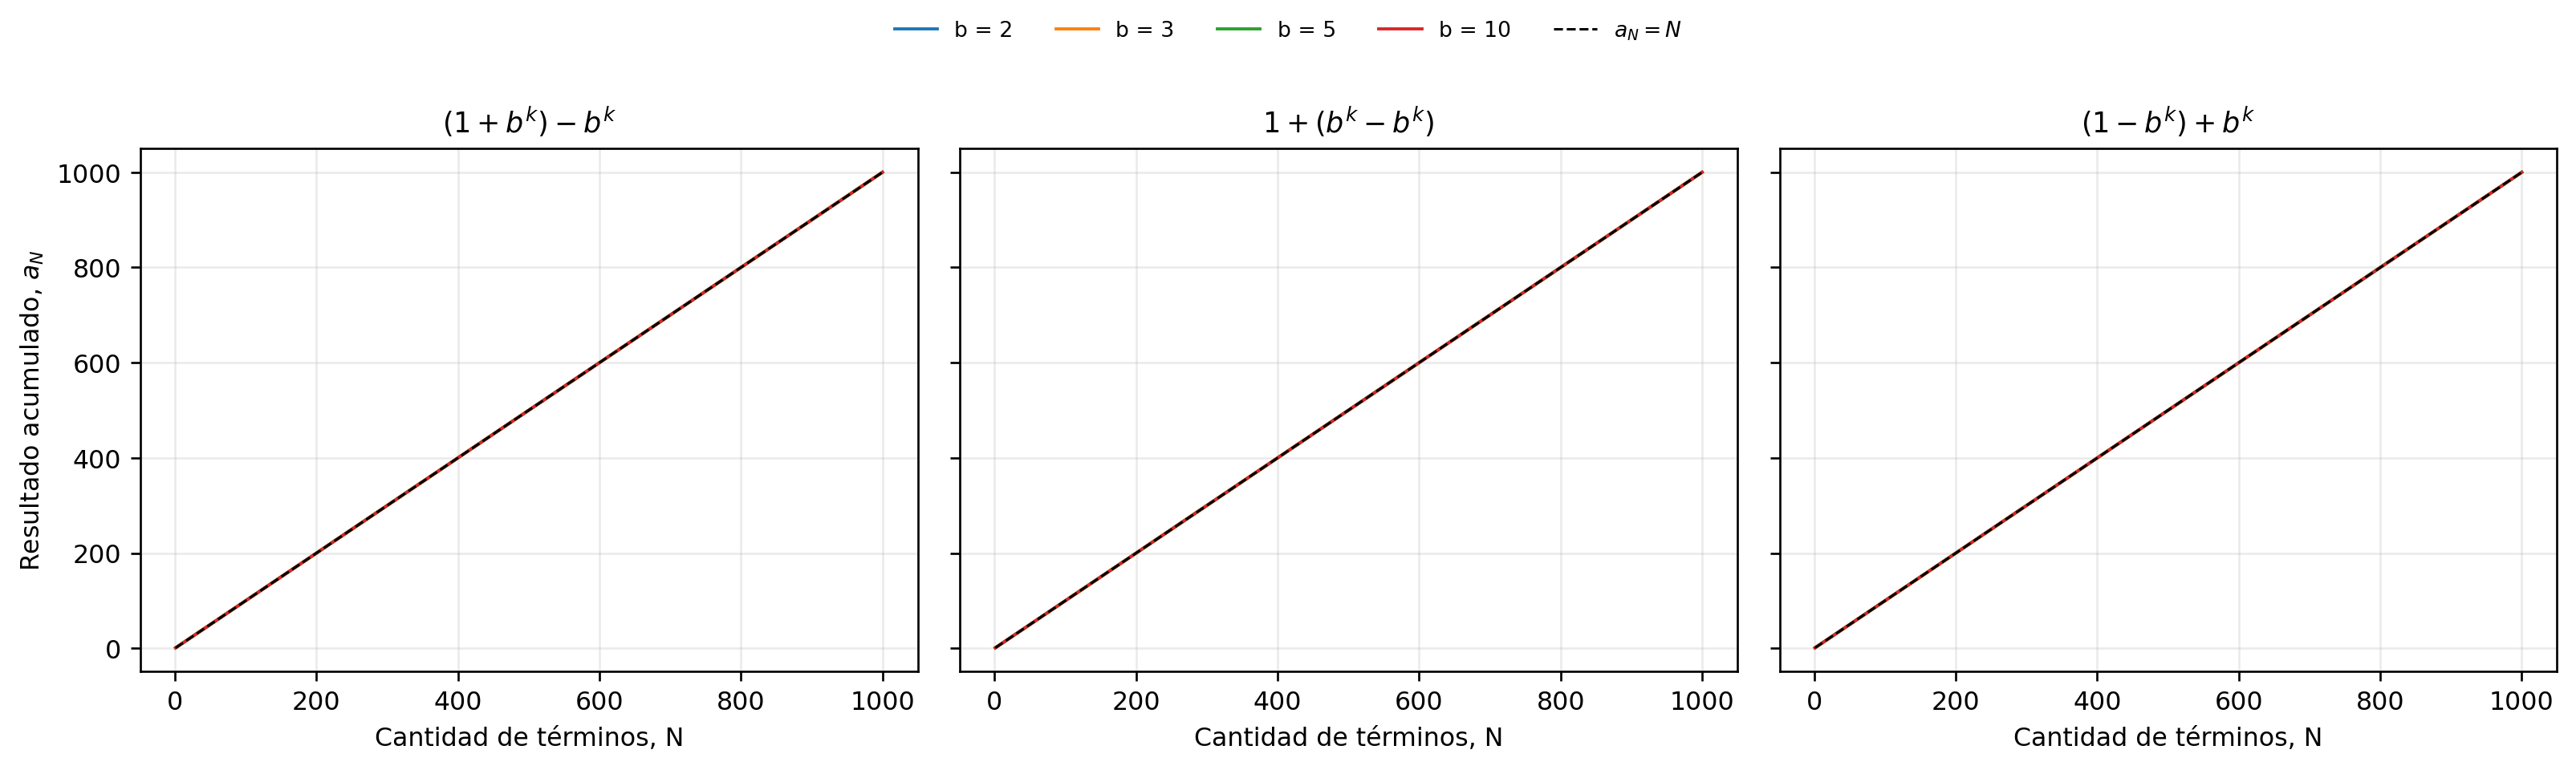
\includegraphics[width=\textwidth]{asociatividad_int.png}
  \caption{Tres asociaciones de $a_N$ con $b=2,3,5,10$ de tipo \codigo{int} y $N=1,\ldots,1000$. Todas las curvas coinciden con la referencia discontinua $a_N=N$.}
  \label{fig:asoc-int}
\end{figure}

Con \codigo{float}, las asociaciones exteriores dejaron de crecer antes del desbordamiento. La asociación central permaneció sobre la referencia mientras $b^k$ fue finito. La Tabla~\ref{tab:asoc-float} y la Figura~\ref{fig:asoc-float} resumen el comportamiento.

\begin{table}[H]
\centering
\caption{Primera desviación y último $N$ finito con bases positivas \codigo{float}.}
\label{tab:asoc-float}
\begin{tabular}{rrrrr}
\toprule
$b$ & $(1+b^k)-b^k$ & $1+(b^k-b^k)$ & $(1-b^k)+b^k$ & Último finito \\
\midrule
2,0  & 53 & --  & 54 & 1000 \\
3,0  & 34 & 647 & 34 & 646 \\
5,0  & 23 & 442 & 23 & 441 \\
10,0 & 16 & 309 & 16 & 308 \\
\bottomrule
\end{tabular}
\begin{minipage}{0.92\textwidth}\footnotesize\emph{Nota.} El guion indica que no hubo desviación en el rango. En la asociación central, la primera desviación coincide con la aparición de \codigo{NaN}. Fuente: \codigo{datos/asociatividad.csv}.\end{minipage}
\end{table}

\begin{figure}[H]
  \centering
  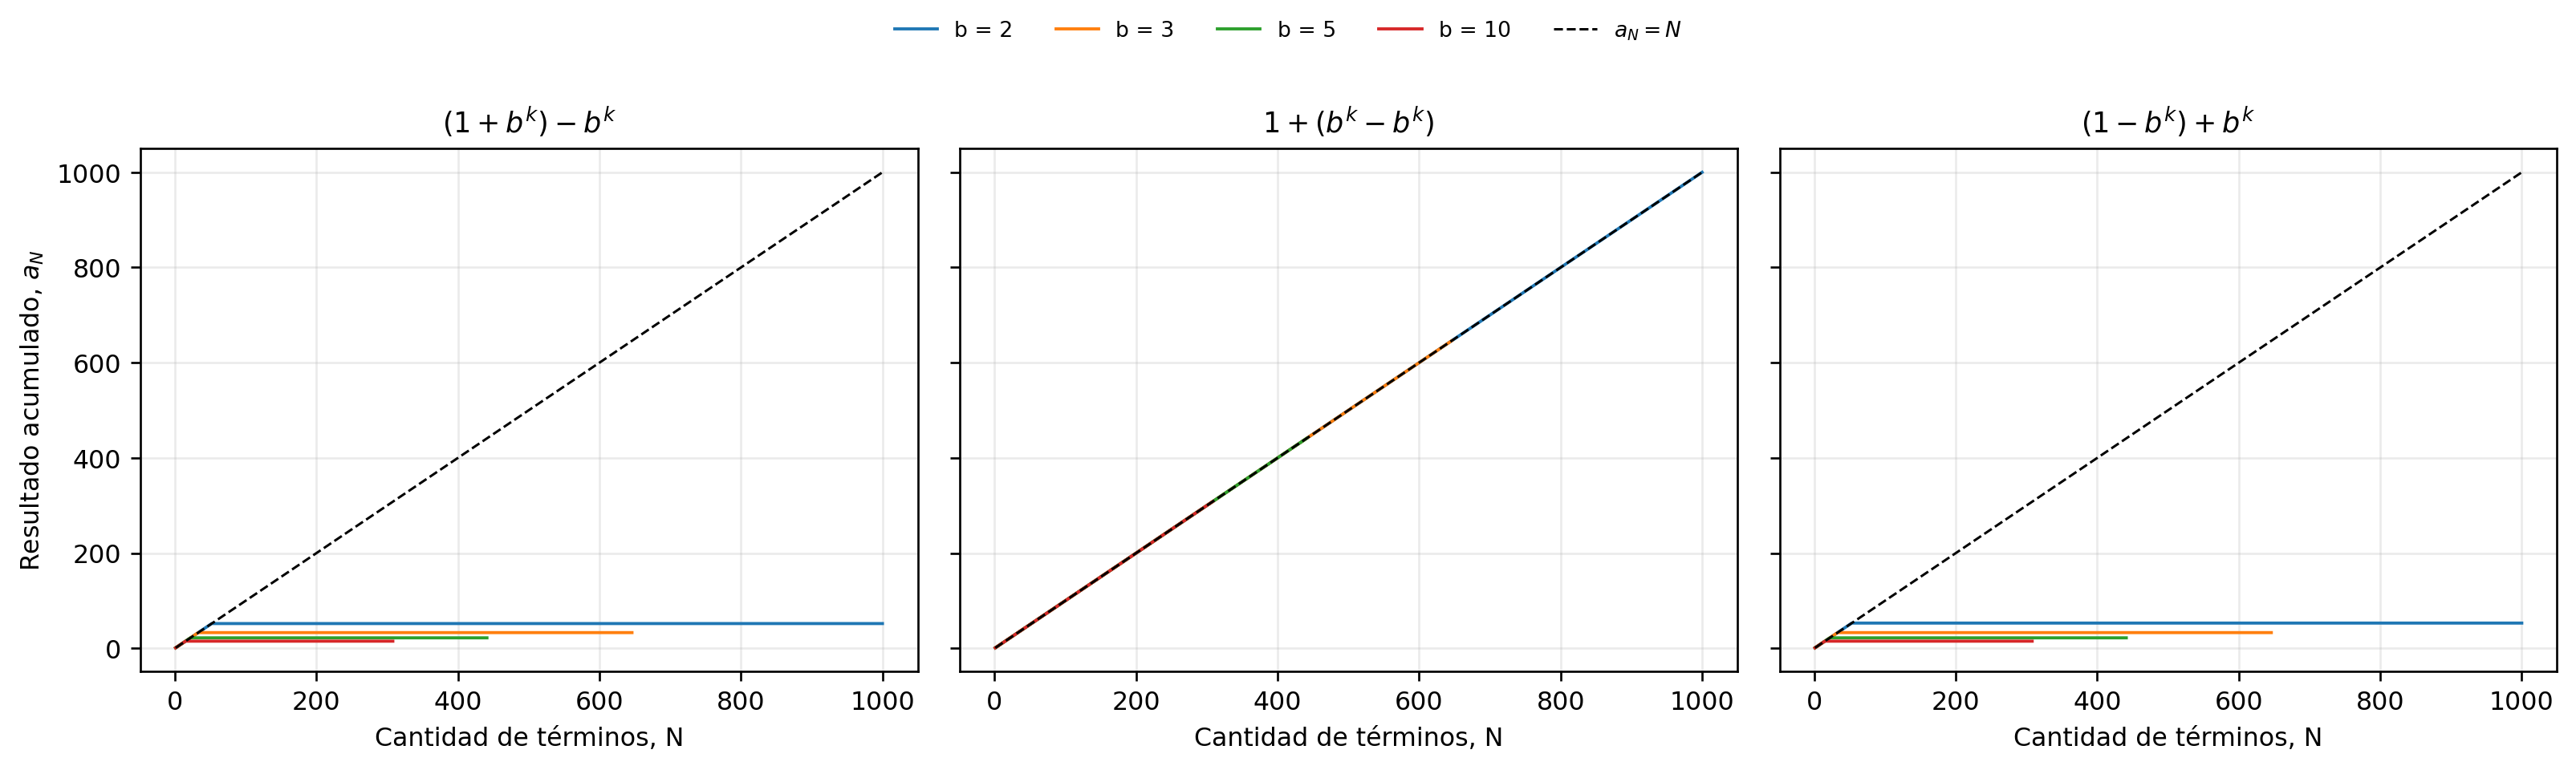
\includegraphics[width=\textwidth]{asociatividad_float.png}
  \caption{Tres asociaciones de $a_N$ con bases positivas \codigo{float}. Las interrupciones de las curvas para $b=3,5,10$ corresponden a valores no finitos, no a datos omitidos.}
  \label{fig:asoc-float}
\end{figure}

Para $b=-2$, los resultados finales de las asociaciones exteriores fueron 53 y 52, en orden inverso al caso $b=2$ (52 y 53). Las demás bases negativas crecientes en módulo también reprodujeron las desviaciones y los límites finitos de sus valores absolutos (Figura~\ref{fig:asoc-neg}). Para $-1\le b\le1$, las tres asociaciones dieron $a_{1000}=1000$.

\begin{figure}[H]
  \centering
  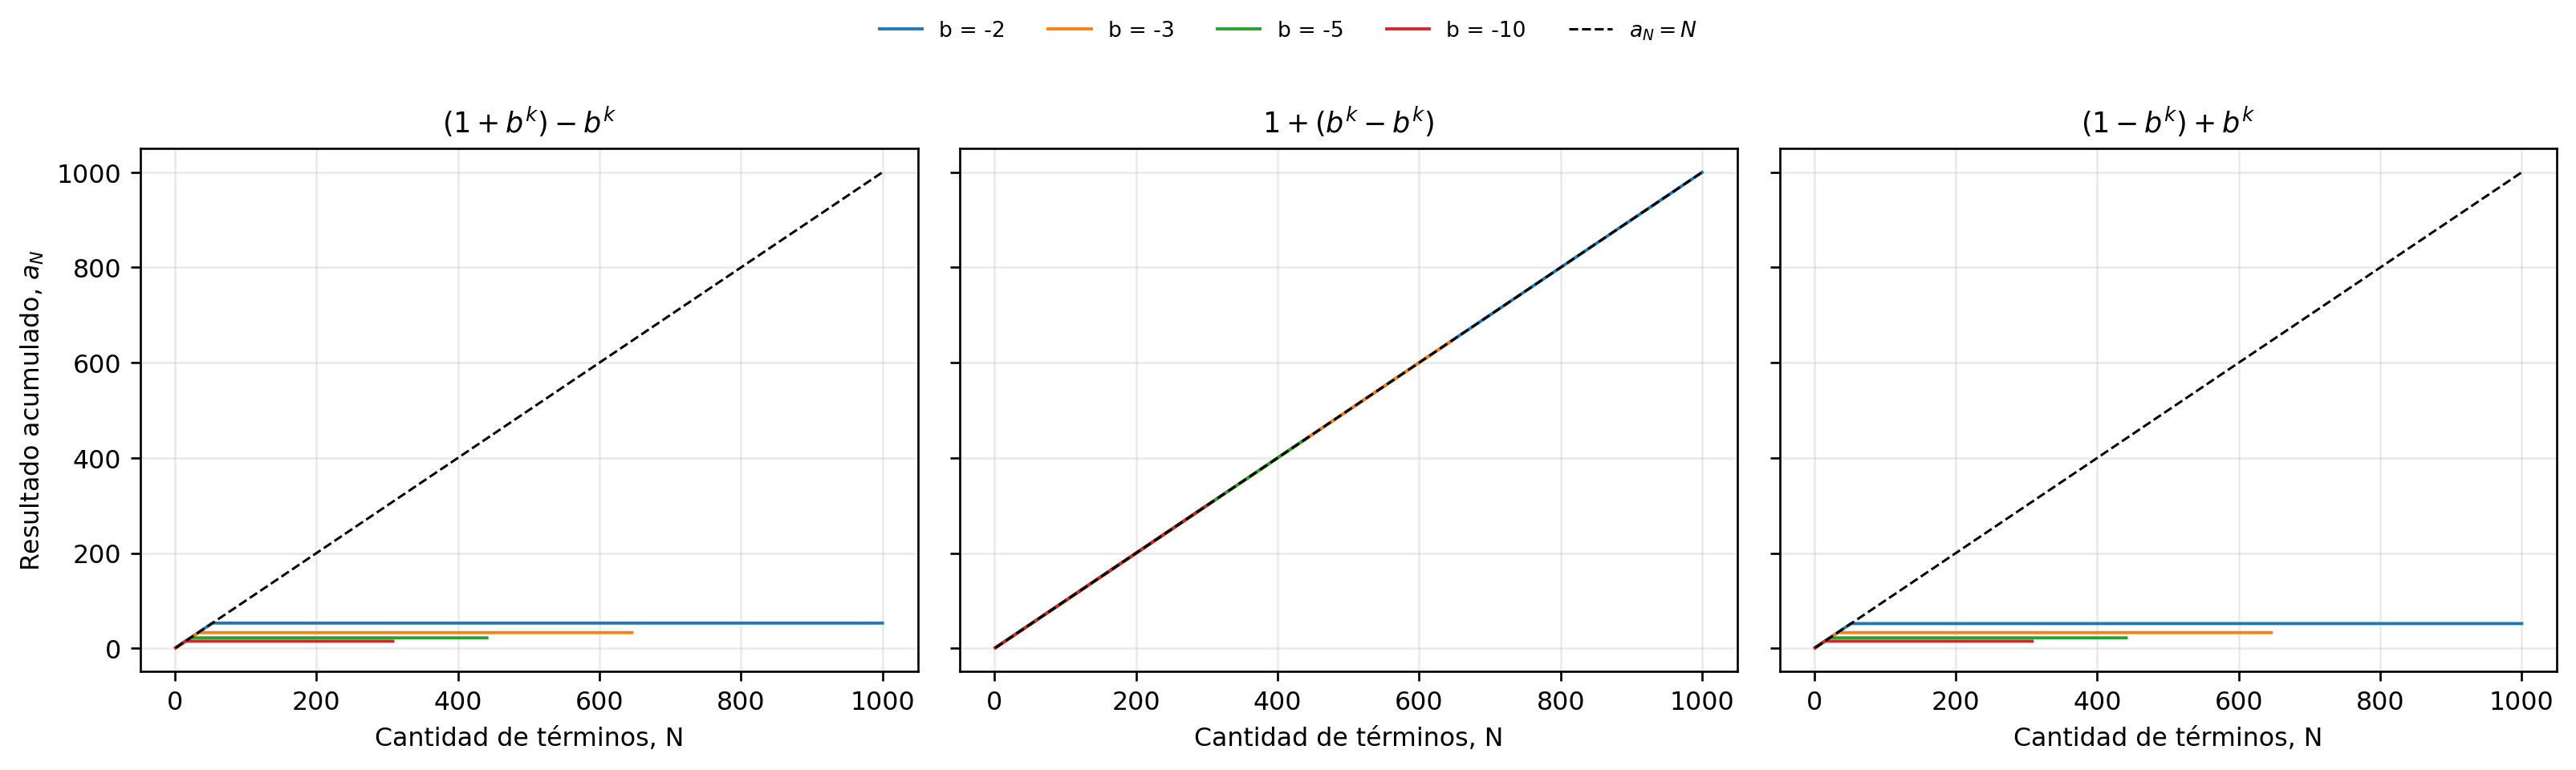
\includegraphics[width=\textwidth]{asociatividad_negativa.png}
  \caption{Tres asociaciones de $a_N$ con $b=-2,-3,-5,-10$ de tipo \codigo{float}. La alternancia de signo intercambia cuál asociación exterior conserva la unidad en el umbral para $|b|=2$.}
  \label{fig:asoc-neg}
\end{figure}

La Tabla~\ref{tab:enteros} presenta el bonus de enteros fijos. Python conservó el resultado y representó $10^{1000}$ con 3322 bits. Los tipos fijos no pudieron representar esa potencia; el acumulador \codigo{int8} además desbordó al intentar almacenar 1000 y terminó en $-24$.

\begin{table}[H]
\centering
\caption{Resultado para $N=1000$, $b=10$ con enteros de distinta capacidad.}
\label{tab:enteros}
\begin{tabular}{lrrrr}
\toprule
Tipo & Bits & $A_N$ & $B_N$ & $C_N$ \\
\midrule
Python \codigo{int} & variable & 1000 & 1000 & 1000 \\
\codigo{int8}  & 8  & -24 & -24 & -24 \\
\codigo{int32} & 32 & 1000 & 1000 & 1000 \\
\codigo{int64} & 64 & 1000 & 1000 & 1000 \\
\bottomrule
\end{tabular}
\par\smallskip
\begin{minipage}{0.92\textwidth}\footnotesize\emph{Nota.} Las potencias intermedias de los tipos NumPy se calcularon con aritmética modular. El resultado 1000 cabe en 32 y 64 bits; no cabe en 8 bits. Fuente: \codigo{datos/enteros\_fijos.csv}.\end{minipage}
\end{table}

\subsection{Influencia del orden de suma}

En el rango corto, los errores se mantuvieron entre cero y unos pocos múltiplos de $10^{-15}$ (Figura~\ref{fig:orden-corto}). En el rango largo, el orden natural y el aleatorio alcanzaron el orden de $10^{-14}$, mientras el orden inverso y Kahan quedaron en cero o cerca de $10^{-16}$ (Figura~\ref{fig:orden-largo}).

\begin{table}[H]
\centering
\caption{Error relativo de los cuatro métodos en valores representativos de $N$.}
\label{tab:orden}
\small
\begin{tabular}{rcccc}
\toprule
$N$ & Mayor a menor & Menor a mayor & Aleatoria & Kahan \\
\midrule
10        & 0 & 0 & 0 & 0 \\
100       & $3{,}36\times10^{-16}$ & 0 & $1{,}12\times10^{-16}$ & 0 \\
1000      & $6{,}67\times10^{-16}$ & $1{,}11\times10^{-16}$ & $6{,}67\times10^{-16}$ & 0 \\
10000     & $6{,}66\times10^{-16}$ & 0 & $2{,}22\times10^{-15}$ & 0 \\
100000    & $1{,}31\times10^{-14}$ & $1{,}11\times10^{-16}$ & $8{,}88\times10^{-15}$ & $1{,}11\times10^{-16}$ \\
1000000   & $4{,}76\times10^{-14}$ & 0 & $3{,}28\times10^{-14}$ & 0 \\
\bottomrule
\end{tabular}
\begin{minipage}{0.95\textwidth}\footnotesize\emph{Nota.} Los ceros son valores originales. La columna aleatoria corresponde a las semillas de cada barrido. Fuentes: \codigo{datos/orden\_10\_a\_10000.csv} y \codigo{datos/orden\_1000\_a\_1000000.csv}.\end{minipage}
\end{table}

\begin{figure}[H]
  \centering
  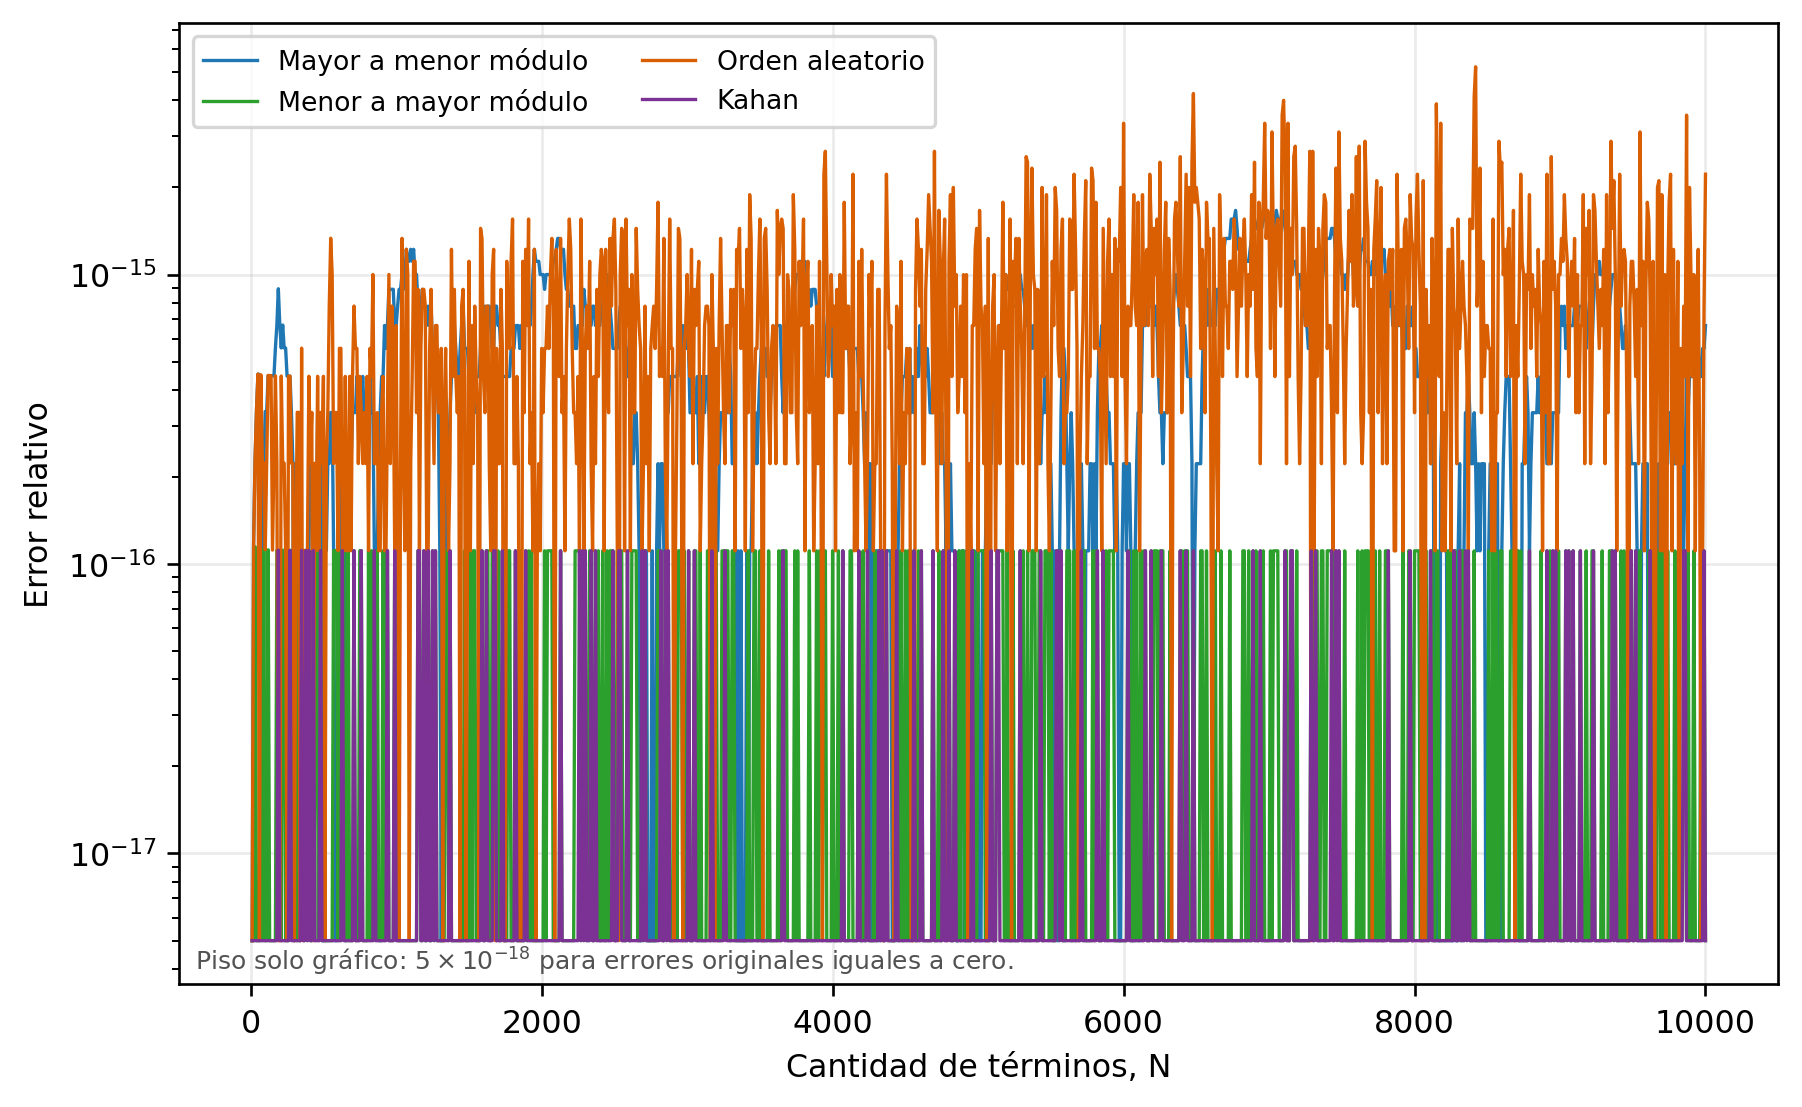
\includegraphics[width=0.89\textwidth]{orden_error_10_a_10000.png}
  \caption{Error relativo para $N=10,20,\ldots,10000$. El eje vertical es logarítmico. Los errores originales iguales a cero se dibujan en $5\times10^{-18}$ solo para hacerlos visibles.}
  \label{fig:orden-corto}
\end{figure}

\begin{figure}[H]
  \centering
  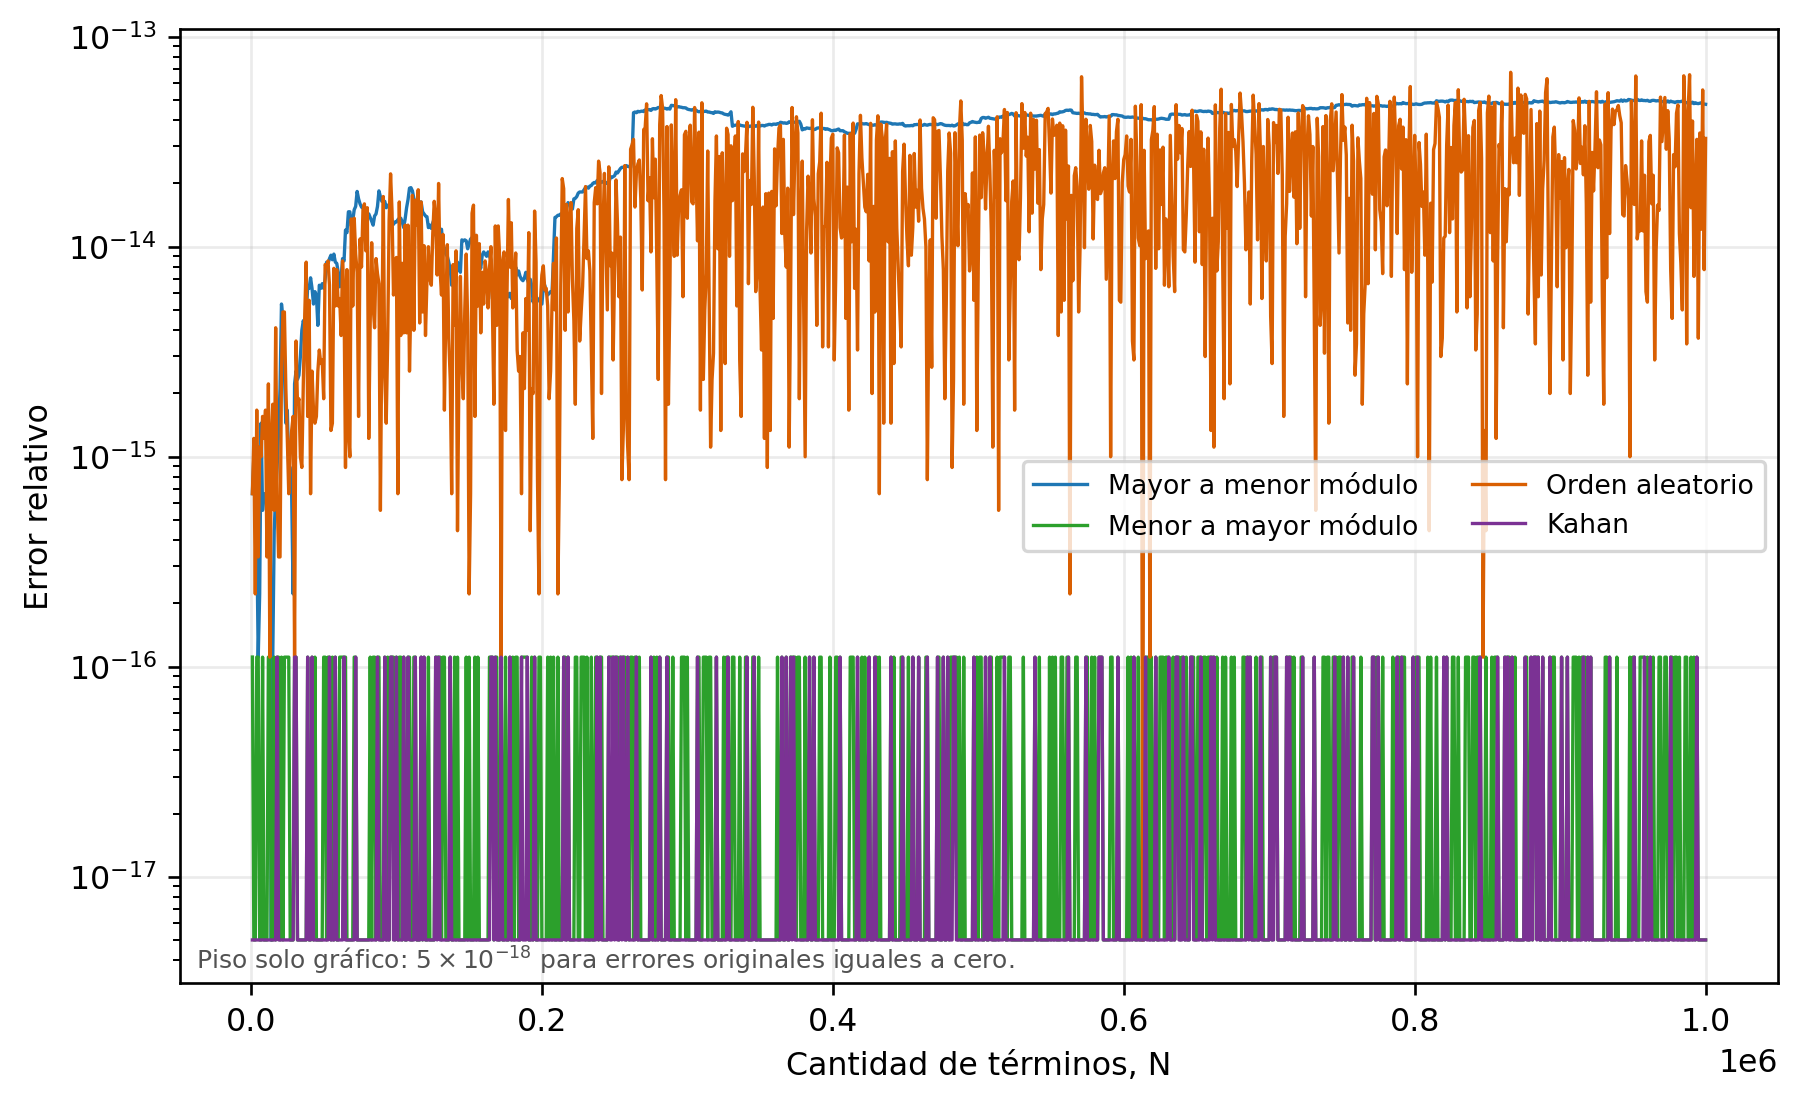
\includegraphics[width=0.89\textwidth]{orden_error_1000_a_1000000.png}
  \caption{Error relativo para $N=1000,2000,\ldots,1000000$. En la escala logarítmica, el piso $5\times10^{-18}$ se aplica únicamente a la representación gráfica de errores nulos.}
  \label{fig:orden-largo}
\end{figure}

Las 30 permutaciones de un millón de términos produjeron 30 errores distintos. El mínimo fue $2{,}22\times10^{-15}$, la mediana $2{,}31\times10^{-14}$ y el máximo $6{,}13\times10^{-14}$. La dispersión se aprecia en la Figura~\ref{fig:repeticiones}.

\begin{figure}[H]
  \centering
  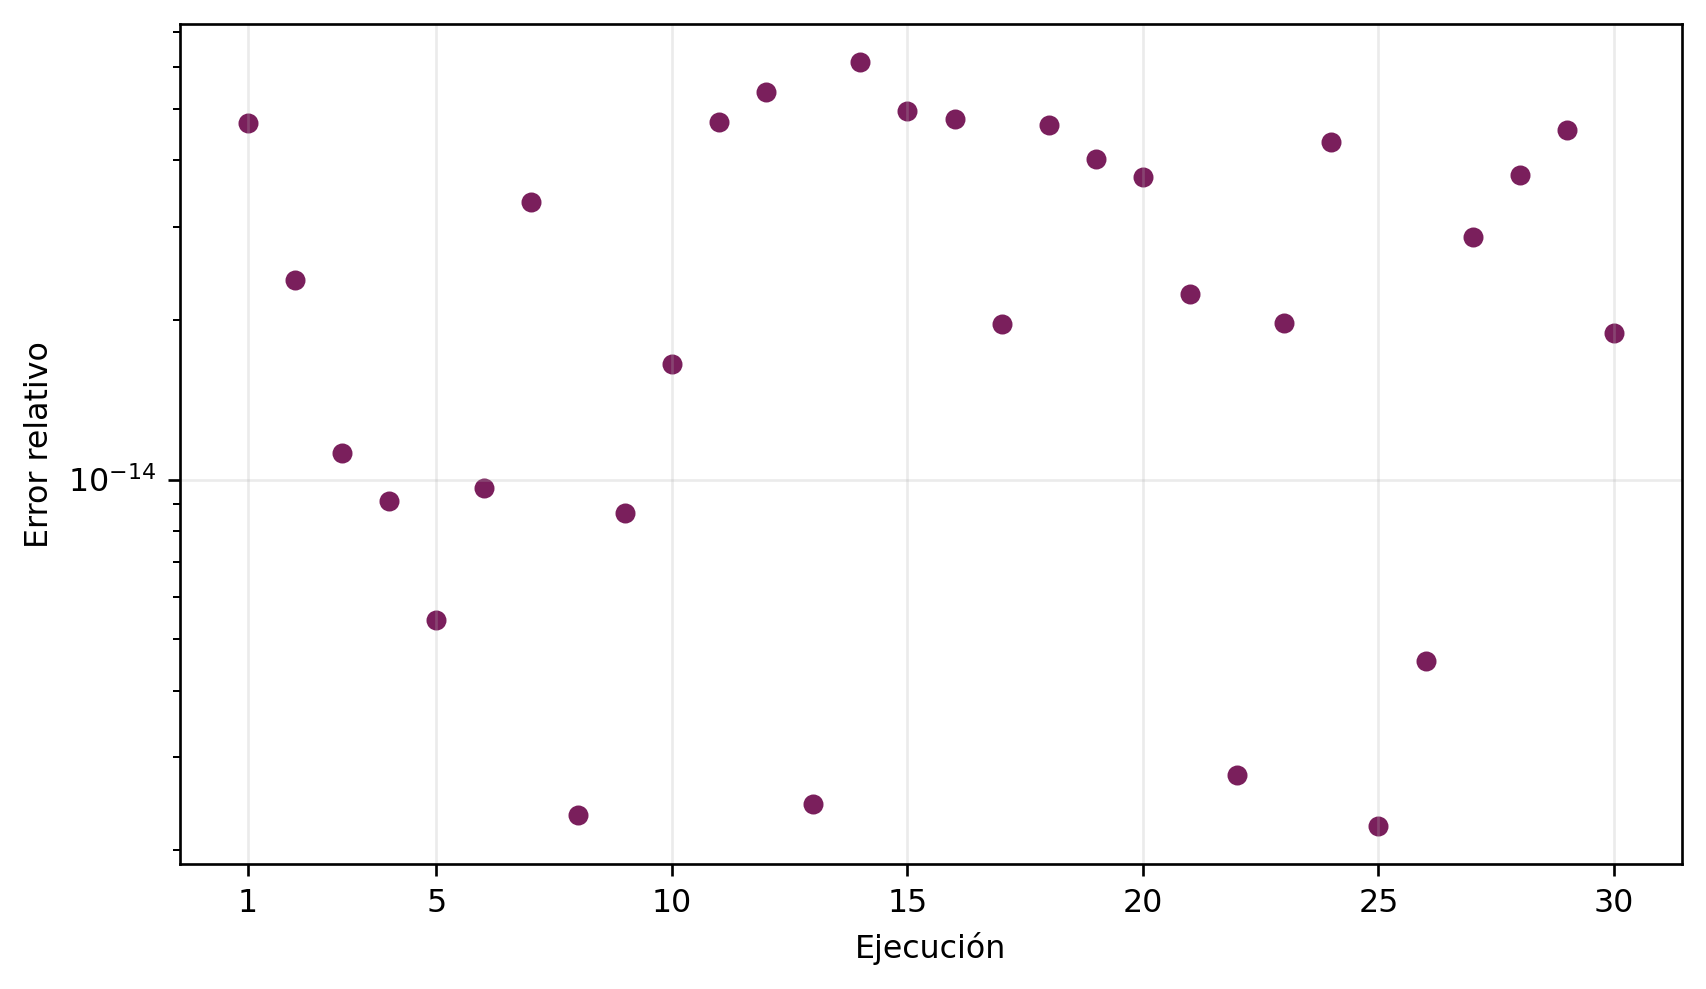
\includegraphics[width=0.84\textwidth]{orden_random_repeticiones.png}
  \caption{Error relativo de 30 permutaciones para $N=10^6$. Cada punto usa una semilla distinta entre 20260914 y 20260943; el eje vertical es logarítmico.}
  \label{fig:repeticiones}
\end{figure}

\subsection{Representaciones de \texorpdfstring{$b_N$}{bN}}

Las dos formas de la Ecuación~\ref{eq:brep} tuvieron errores cercanos al épsilon de máquina, pero no coincidieron para todos los $N$. Ninguna fue uniformemente mejor. Para $N=10000$, los errores fueron $6{,}66\times10^{-16}$ en la forma directa y $3{,}33\times10^{-16}$ en la telescópica. La alternancia y los ceros del rango completo se muestran en la Figura~\ref{fig:brep}.

\begin{figure}[H]
  \centering
  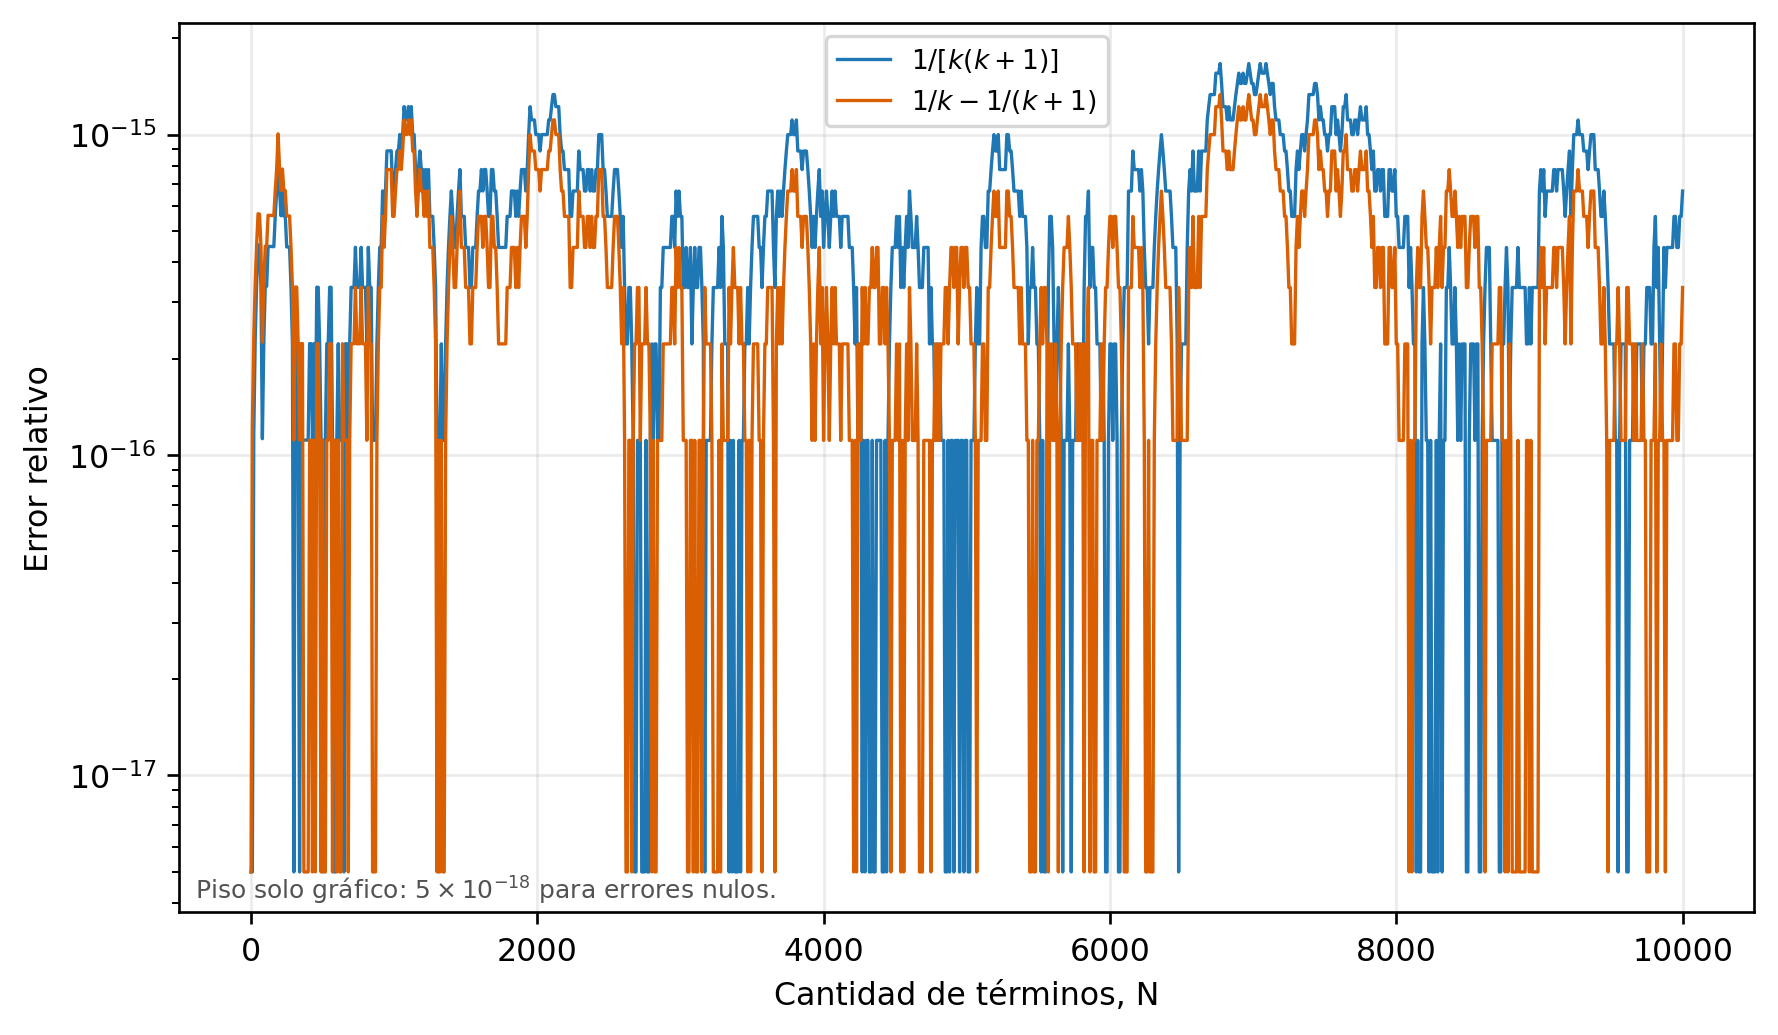
\includegraphics[width=0.86\textwidth]{representaciones_b_error.png}
  \caption{Error relativo de las dos sumatorias de $b_N$ para $N=1,10,20,\ldots,10000$. Los ceros originales se muestran en el piso gráfico $5\times10^{-18}$.}
  \label{fig:brep}
\end{figure}

Las formas cerradas también difirieron por una ulp en ciertos valores. Para $N=2^{53}$, $1-1/(N+1)$ dio $0{,}9999999999999999$, mientras $N/(N+1)$ se redondeó a 1. La Figura~\ref{fig:bonus-b} ubica las diferencias no nulas y marca $2^{53}$.

\begin{figure}[H]
  \centering
  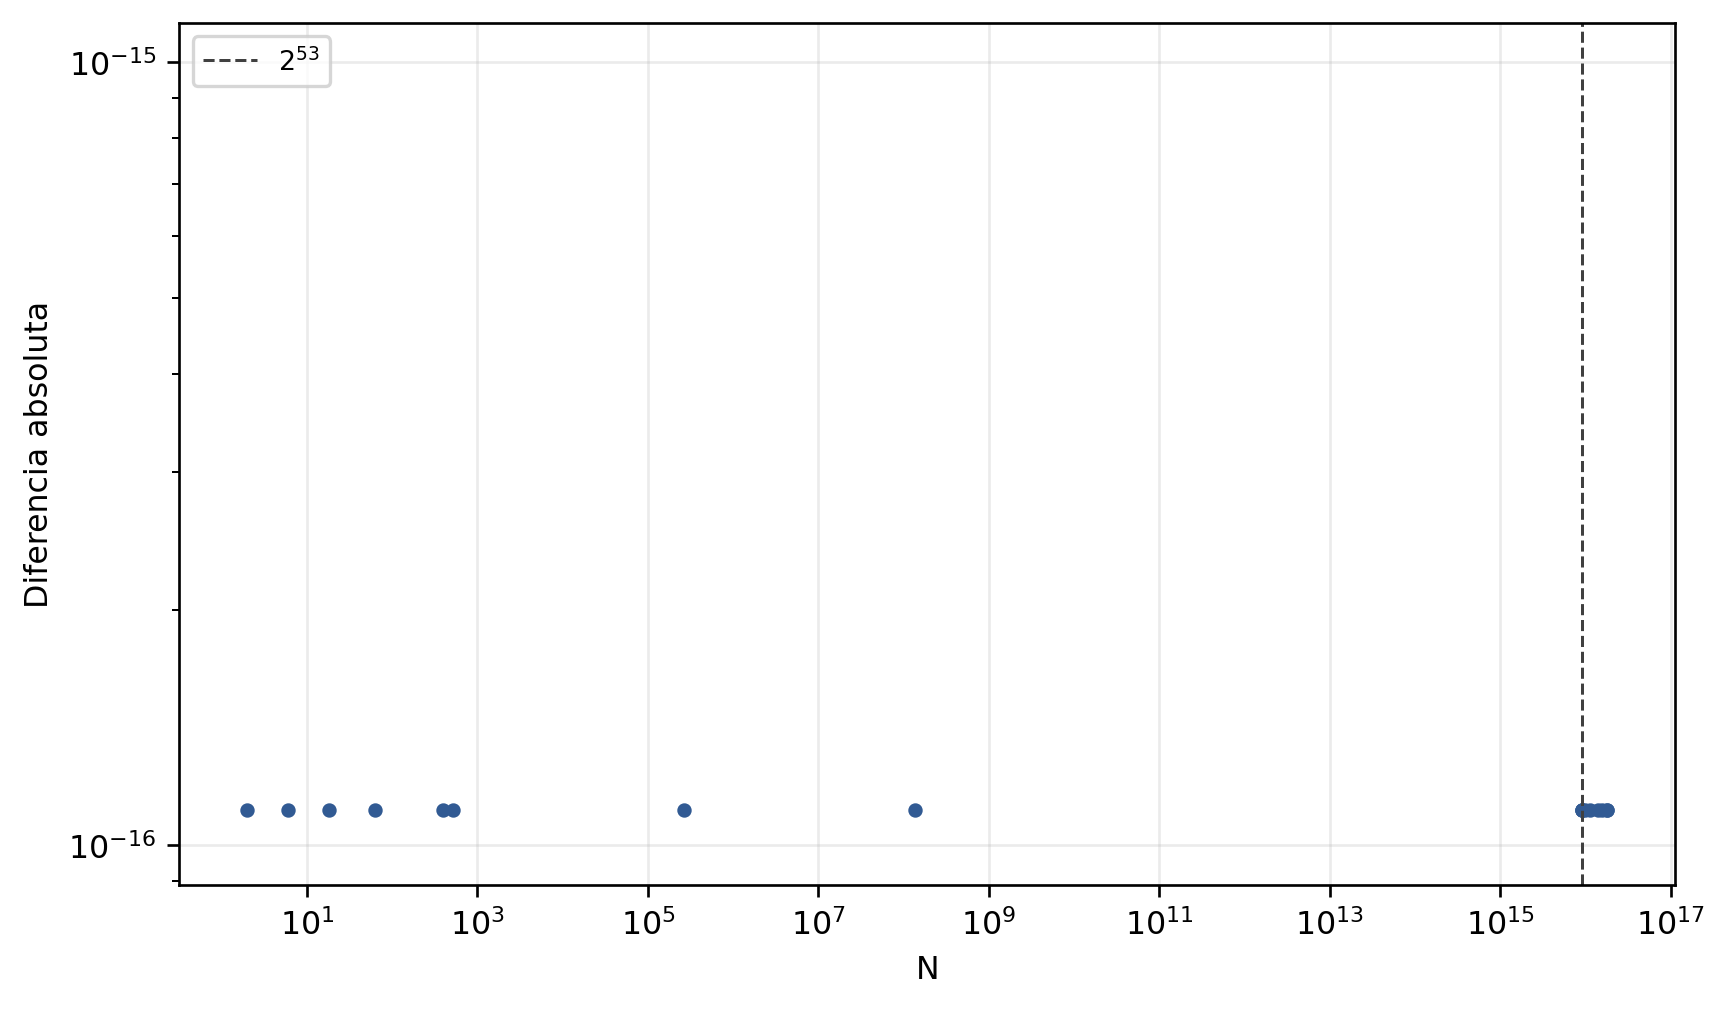
\includegraphics[width=0.84\textwidth]{bonus_b_formas_cerradas.png}
  \caption{Diferencias no nulas entre $1-1/(N+1)$ y $N/(N+1)$ hasta $10^{18}$. Ambos ejes son logarítmicos; la línea discontinua marca $N=2^{53}$. Los valores sin diferencia no se dibujan.}
  \label{fig:bonus-b}
\end{figure}

\subsection{Representaciones de \texorpdfstring{$c_N$}{cN}}

La diferencia absoluta entre las dos formas de $c_N$ aumentó en términos generales, aunque presentó compensaciones locales. La Tabla~\ref{tab:crep} contiene valores tomados del CSV y la Figura~\ref{fig:crep} muestra el rango completo.

\begin{table}[H]
\centering
\caption{Valores de las dos representaciones de $c_N$ y diferencia absoluta.}
\label{tab:crep}
\small
\begin{tabular}{rccc}
\toprule
$N$ & $c_N^{(1)}$ racionalizada & $c_N^{(2)}$ sustractiva & $D_N$ \\
\midrule
1     & 0,4142135624 & 0,4142135624 & $5{,}55\times10^{-17}$ \\
10    & 1,3560331890 & 1,3560331890 & $2{,}22\times10^{-16}$ \\
100   & 2,4846796649 & 2,4846796649 & $6{,}22\times10^{-15}$ \\
1000  & 3,6337202111 & 3,6337202111 & $1{,}79\times10^{-13}$ \\
10000 & 4,7847877371 & 4,7847877371 & $2{,}85\times10^{-11}$ \\
\bottomrule
\end{tabular}
\begin{minipage}{0.92\textwidth}\footnotesize\emph{Nota.} Las columnas centrales se muestran con diez decimales; $D_N$ fue calculada con los valores completos. Fuente: \codigo{datos/representaciones.csv}.\end{minipage}
\end{table}

\begin{figure}[H]
  \centering
  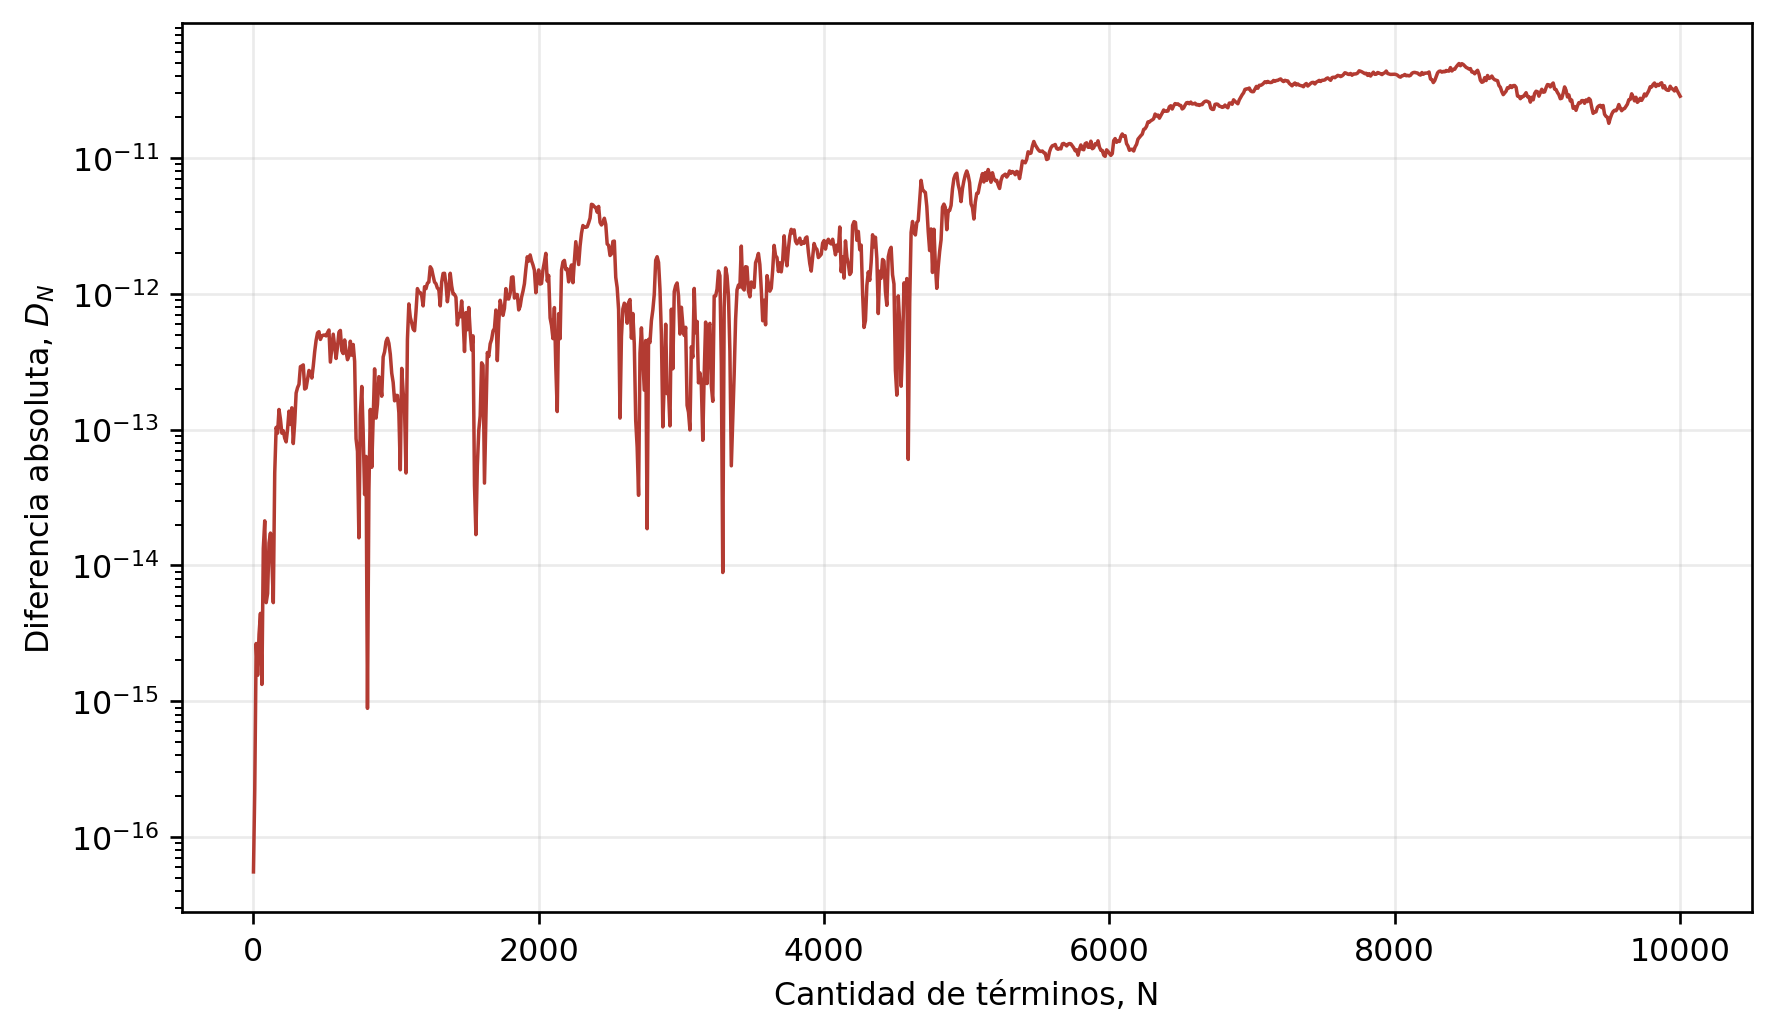
\includegraphics[width=0.86\textwidth]{representaciones_c_diferencia.png}
  \caption{Diferencia absoluta $D_N$ entre las dos sumatorias de $c_N$ para $N=1,10,20,\ldots,10000$. El eje vertical es logarítmico.}
  \label{fig:crep}
\end{figure}

El error relativo del término sustractivo alcanzó por primera vez $10^{-12}$ en $k=87$, $10^{-8}$ en $k=8193$ y $10^{-4}$ en $k=860284$. El primer cero apareció en $k=67108864=2^{26}$, aunque el término matemático y la forma racionalizada seguían siendo positivos (Figura~\ref{fig:bonus-c}).

\begin{figure}[H]
  \centering
  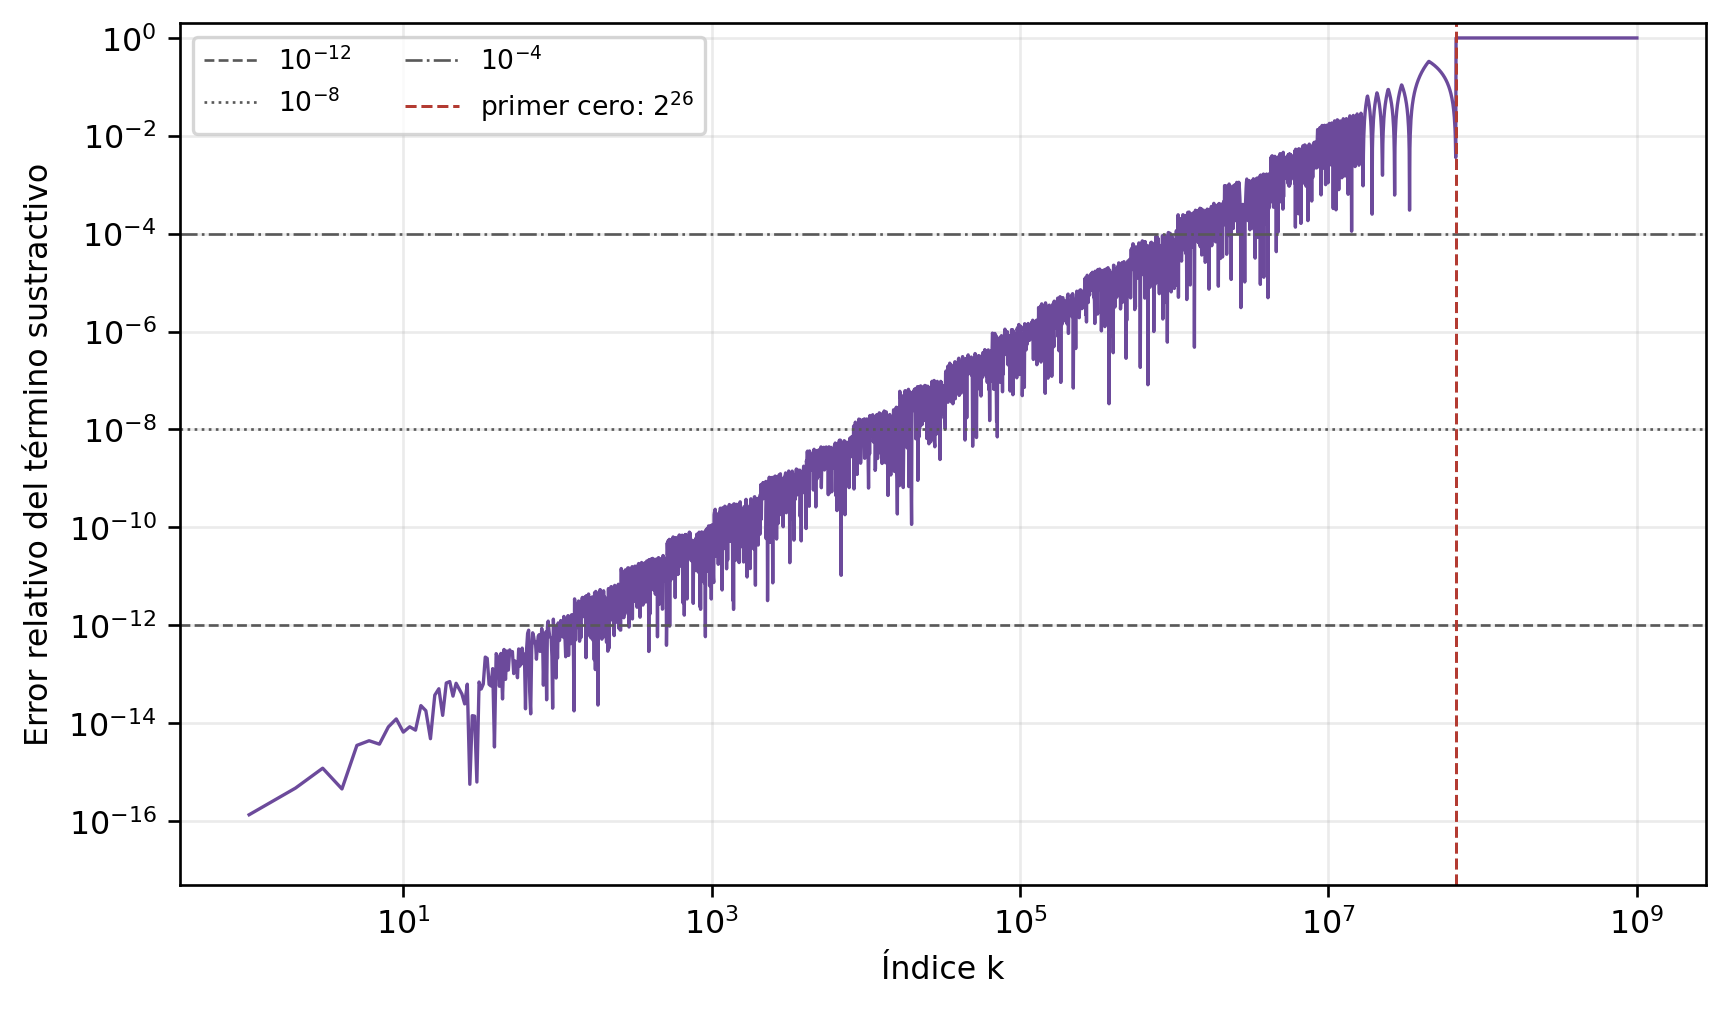
\includegraphics[width=0.86\textwidth]{bonus_c_terminos.png}
  \caption{Error relativo de $\sqrt{k^2+1}-k$ respecto de la forma racionalizada. Las líneas horizontales indican los tres umbrales y la vertical marca el primer término sustractivo redondeado a cero. Ambos ejes son logarítmicos.}
  \label{fig:bonus-c}
\end{figure}

\section{Discusión}

\subsection{Pérdida de la unidad, infinito y \codigo{NaN}}

El contraste entre \codigo{int} y \codigo{float} se explica por su representación. Los enteros de Python tienen precisión arbitraria y crecen mientras haya memoria disponible \citep{pythonint2026}; por eso el mismo valor exacto de $b^k$ se suma y se resta. En \codigo{binary64}, la precisión es fija. Para $b=2$, $(1+2^{53})-2^{53}$ vale cero numéricamente porque $2^{53}+1$ se redondea a $2^{53}$. En la tercera asociación, $2^{53}-1$ aún es representable y se conserva un término adicional; desde el paso siguiente también se pierde la unidad.

La asociación $1+(b^k-b^k)$ es más estable porque cancela dos representaciones idénticas antes de incorporar la unidad. Su límite no es la precisión del significando sino el rango del exponente. Cuando la potencia excede el máximo finito se obtiene infinito; después, $\infty-\infty$ es una operación indeterminada y produce \codigo{NaN}. Como cualquier operación posterior con ese valor sigue dando \codigo{NaN}, las curvas quedan interrumpidas.

\subsection{Bases negativas, \texorpdfstring{$b\le1$}{b menor o igual a 1} y enteros fijos}

Para $0\le b\le1$, la magnitud de $b^k$ no crece y la unidad no queda por debajo de su resolución. El mismo razonamiento vale para $-1\le b<0$. Sin embargo, la condición literal $b\le1$ también incluye $b<-1$. Allí $|b|^k$ crece y el fenómeno reaparece. La alternancia de signo cambia si cada asociación exterior suma o resta la unidad respecto de una potencia positiva o negativa; por eso $b=-2$ intercambia los resultados de $b=2$.

Los enteros fijos muestran otro mecanismo. Sus potencias desbordan, pero bajo aritmética modular las identidades $(1+x)-x\equiv1$ se conservan. El problema visible en \codigo{int8} aparece al acumular 1000 unos: $1000$ módulo $256$ es $232$, interpretado con signo como $-24$. En otros lenguajes el desbordamiento puede lanzar una excepción, envolver modularmente o quedar sin comportamiento definido; no debe generalizarse el comportamiento particular de NumPy.

\subsection{Orden, Kahan y variabilidad aleatoria}

Los términos $1/[k(k+1)]$ son positivos y decrecientes. En el orden natural el acumulador se aproxima rápidamente a 1; los términos finales son demasiado pequeños respecto de su ulp y parte de su contribución se pierde. En el orden inverso, los términos pequeños se combinan cuando el acumulador también es pequeño. Esto explica la diferencia de más de dos órdenes de magnitud observada para $N=10^6$.

Kahan consigue una precisión semejante sin invertir la secuencia. La compensación de la Ecuación~\ref{eq:kahan} conserva una estimación de lo descartado y la reincorpora en iteraciones siguientes. El cero medido no prueba exactitud real: significa que el resultado final coincide con el \codigo{float64} de $N/(N+1)$.

Cada permutación aleatoria define una secuencia distinta de acumuladores y redondeos. Por eso los mismos términos generaron 30 errores diferentes. La semilla vuelve reproducible cada permutación, pero no elimina la variabilidad cuando cambia el orden. El rango observado también muestra que una permutación casual puede superar o empeorar el orden natural sin ofrecer una garantía sistemática.

\subsection{Representaciones de \texorpdfstring{$b_N$}{bN}}

La forma directa de cada término realiza una multiplicación y una división. La forma telescópica realiza dos divisiones y una resta de valores cercanos. Sus redondeos intermedios son diferentes, por lo que no hay obligación de coincidencia bit a bit. En este rango, ambos errores quedaron cerca del épsilon y se alternaron: el experimento no respalda declarar una de las dos sumatorias uniformemente superior.

El bonus cerrado revela otra sutileza. Cerca de $2^{53}$, convertir $N$ y $N+1$ a \codigo{float64} puede eliminar su diferencia antes de dividir. En $N/(N+1)$ ambos se redondearon al mismo valor y el cociente fue 1. En $1-1/(N+1)$ la pequeña corrección todavía produjo el \codigo{float64} inmediatamente inferior a 1. Con valores aún mayores, esa corrección cae por debajo de media ulp y las dos formas terminan en 1.

\subsection{Cancelación en \texorpdfstring{$c_N$}{cN}}

Para $k$ grande,
\begin{equation}
\sqrt{k^2+1}=k\sqrt{1+k^{-2}}\approx k+\frac{1}{2k}.
\end{equation}
La forma sustractiva intenta recuperar una cantidad cercana a $1/(2k)$ restando dos operandos de tamaño $k$. Los dígitos principales se cancelan y los errores de la raíz quedan amplificados. La forma racionalizada calcula directamente una cantidad pequeña y positiva; mantiene la escala del resultado y evita la resta problemática.

Los umbrales confirmados muestran una progresión coherente: desde $k=8193$ la forma sustractiva ya perdió al menos ocho cifras relativas. En $2^{26}$, el cálculo de $k^2+1$ y su raíz se redondeó de modo que la raíz resultó igual a $k$; la resta dio cero y eliminó por completo un término positivo. Las oscilaciones de $D_N$ no contradicen la inestabilidad, porque errores sucesivos pueden tener signos opuestos y compensarse parcialmente.

\subsection{Limitaciones}

Los resultados corresponden al entorno documentado. IEEE 754 favorece la portabilidad, pero el último bit de \codigo{sqrt} o de ciertas optimizaciones puede cambiar entre bibliotecas. Además, $N/(N+1)$ también es una aproximación \codigo{float64}; el error relativo compara dos números en la misma precisión. Una validación futura podría utilizar racionales exactos o precisión múltiple.

Para $c_N$, la consigna solicita comparar dos implementaciones, no calcular el error verdadero de cada una. La racionalización permite identificar la forma más estable, pero una referencia de alta precisión cuantificaría ambos errores por separado. Por último, 30 permutaciones prueban variabilidad, aunque no describen la distribución de todos los $N!$ órdenes posibles.

\section{Conclusiones}

Los experimentos cumplieron el objetivo de mostrar que las propiedades algebraicas no se trasladan automáticamente a la aritmética computacional. La precisión finita obliga a redondear cada resultado intermedio y hace que el tipo, la asociación y el orden formen parte efectiva del algoritmo.

En asociatividad, los enteros arbitrarios de Python preservaron $a_N=N$, mientras \codigo{float64} perdió unidades y luego produjo valores no finitos. La asociación que cancela primero $b^k-b^k$ fue más estable hasta el desbordamiento. Las bases negativas demostraron que importa el crecimiento de $|b|$, no solo la desigualdad $b\le1$, y los tipos fijos mostraron que la exactitud entera depende de no exceder el rango disponible.

En la suma de $b_N$, procesar de menor a mayor y usar Kahan redujo el error frente al orden natural. Las permutaciones aleatorias confirmaron que los mismos sumandos pueden dar distintos resultados. Las dos representaciones sumatorias de $b_N$ quedaron cerca de la precisión de máquina sin una ganadora uniforme, mientras la forma sustractiva de $c_N$ sufrió cancelación catastrófica y llegó a producir términos nulos.

En consecuencia, aumentar $N$ no garantiza una aproximación mejor si el algoritmo descarta información. Una implementación confiable debe elegir conscientemente el tipo numérico, el orden y la forma algebraica. Como línea futura, conviene repetir el estudio con \codigo{float32}, \codigo{longdouble}, precisión arbitraria y suma por pares, comparando precisión, memoria y tiempo.

\clearpage
\bibliographystyle{apalike}
\begingroup
\raggedright
\bibliography{referencias}
\endgroup

\end{document}
